% Figure / table inputs

\chapter{Approach and Custom Software solutions}
\todo[inline]{replace CITEME tags in Approach and Custom Software solutions}

\section{Purpose}
Illustrate how lessons learned in previous chapter (as well as new lessons introduced here) are addressed through custom software solutions.
\begin{enumerate}
 \item RNA-seq analysis, reproducibility, updating
 \item Integration of multiple disparate Omics scale data types
 \item Documentation of exactly how analyses were carried out (IPython notebooks)
\end{enumerate}

\todo[inline]{MEGA: you need to write most of this chapter}

\section{The phylogenetic transcriptional correspondence index (PTCI)}








Look at the parameter space of the PTCI (Figure \ref{fig:ptci-space}).  
\input{figures/ptci-space}

Here is the PTCI calculation:
\begin{equation} \label{eq:ptci}
\mathrm{PTCI} = \left( r_{x} + \frac{r_{t}}{2} \right) \cdot w(d)
\end{equation}

The graph model is useful (Figure \ref{fig:nway-ortholog-graph})


\begin{figure}[hp]
\centering
% 
    \begin{subfigure}[t]{.5\linewidth}
    \centering
    \includegraphics[width=\linewidth]{figures/figs/gfunc_graph_figs/ortho-graph-model.pdf}
    \caption{N-way 1:1 ortholog graph structure}\label{fig:nway-ortholog-graph-model}
    \end{subfigure}%
% 
% 
% 
    \begin{subfigure}[t]{.5\linewidth}
    \centering
    \includegraphics[width=\linewidth]{figures/figs/gfunc_graph_figs/ortho-graph-node-data.pdf}
    \caption{Node data model}\label{fig:nway-ortholog-graph-node-data}
    \end{subfigure}
% 
% 
% 
% 
% 
% 
    \begin{subfigure}[t]{.5\linewidth}
    \centering
    \includegraphics[width=\linewidth]{figures/figs/gfunc_graph_figs/ortho-graph-edge-data.pdf}
    \caption{Edge data model}\label{fig:nway-ortholog-graph-edge-data}
    \end{subfigure}%
% 
% 
%     
    \begin{subfigure}[t]{.5\linewidth}
    \centering
    \includegraphics[width=\linewidth]{figures/figs/gfunc_graph_figs/ortho-graph-ptci.pdf}
    \caption{Example PTCI data}\label{fig:nway-ortholog-graph-ptci}
    \end{subfigure}
% 
% 
% 
\caption[Graph model used to integrate data types]{\sf \textbf{Graph model used to integrate data types.}}\label{fig:nway-ortholog-graph}
\end{figure}


\pagebreak[4]
\section{Blacktie RNA-seq pipeline}

See Figure \ref{fig:tuxedo}




\begin{landscape}
 
 
 \begin{figure}[hp]
\centering
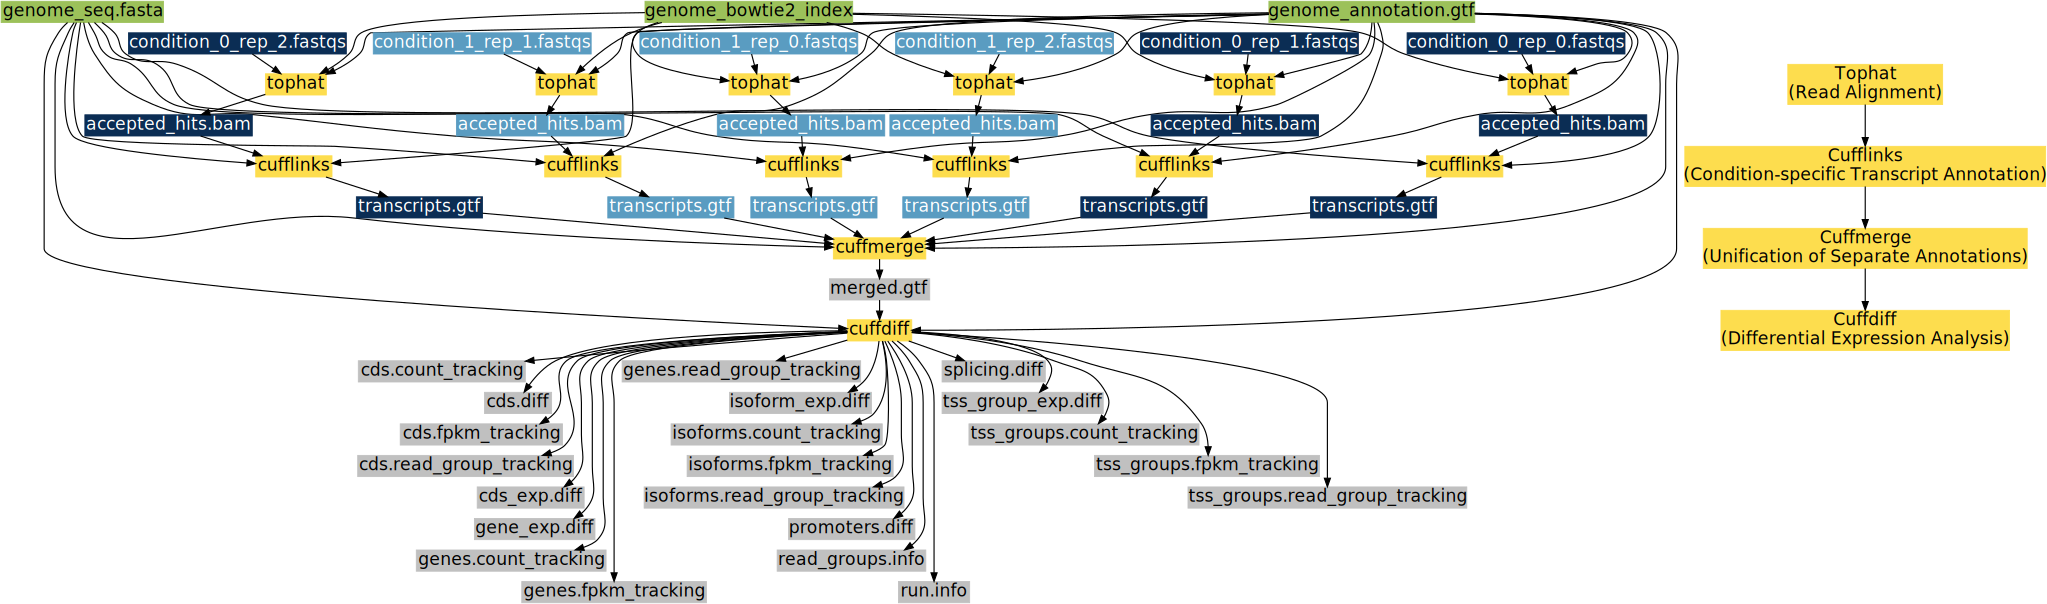
\includegraphics[width=\linewidth]{figures/figs/tuxedo_dot/707354_6/tophat_cufflinks_ins_outs.pdf}
\caption[Diagram of Abbreviated Tophat/Cufflinks Inputs and Outputs]{\textbf{Diagram of Abbreviated Tophat/Cufflinks Inputs and Outputs:}\\
	This figure demonstrates the complexities of a typical RNA-seq experiment as analyzed with the ``Tuxedo Protocol''. It models a fairly \textbf{simple} two condition experiment with each condition having three replications. It is ``abbreviated'' in that it only displays the output files that will be used in the next step for all steps except the \UseVerb{cuffdiff} step. The complete output of \UseVerb{cuffdiff} is included to demonstrate the final challenge of integrating the data which exists in multiple cross-referenced files.\\ 
	(\textsc{Dark Blue} - Inputs/Outputs associated with Condition Zero; 
	\textsc{Light Blue} - Inputs/Outputs associated with Condition One; 
	\textsc{Grey} - Inputs/Outputs associated with Condition Zero \textbf{AND} Condition One; 
	\textsc{Green} - Inputs Specific to the Reference Genome; 
	\textsc{Gold} - Program Calls)
}
	\label{fig:tuxedo}
\end{figure}
 
 
 
\end{landscape}






%%% Local Variables: ***
%%% mode: latex ***
%%% TeX-master: "thesis.tex" ***
%%% End: ***
